\subsection{Oversigt}

Der er valgt at benytte dette view til at vise afhængigheder ifm. de forskellige komponenter og noder. 
Dette virker yderst relevant for at kunne danne et overblik for eventuel videre udvikling.


\begin{figure}[htb]
    \centering
    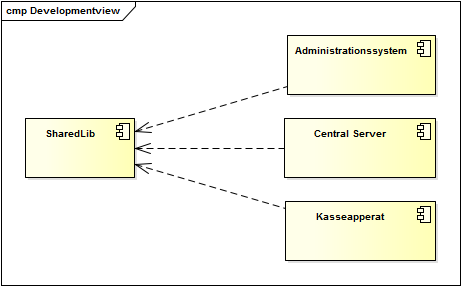
\includegraphics[width=0.8\textwidth]{Systemarkitektur/ImplementeringsView/Billeder/Development.png}
    \caption{Development view for systemet}
    \label{fig:devview}
\end{figure}


På diagrammet i figur \ref{fig:devview} ses det hvordan de tre funktionelle systemer\footnote{\gls{CS} samt \gls{AS} og \gls{KA}} er afhængig af det delte bibliotek \gls{SL}. I dette bibliotek findes datamodeller og kommunikationsprotokoller, som de andre systemer bruger og er afhængige af.\\
En eventuel ændring i \gls{SL}, ville have betydelige konsekvenser for de resterende systemer. Det er derfor vigtigt at gøre sig overvejelser over hvor disse afhængigheder er i systemet, inden man foretager større ændringer. Eksempler på konkrete afhængigheder kunne være:

\begin{itemize}
  \item Produkter
  \item Produktkategorier
\end{itemize}

En reference må da være til stede i alle systemer, som ønsker at arbejde med produkter eller kommunikation i systemet.